\subsection{Imaging systems}\label{subsec:imaging-systems}
\begin{figure}
    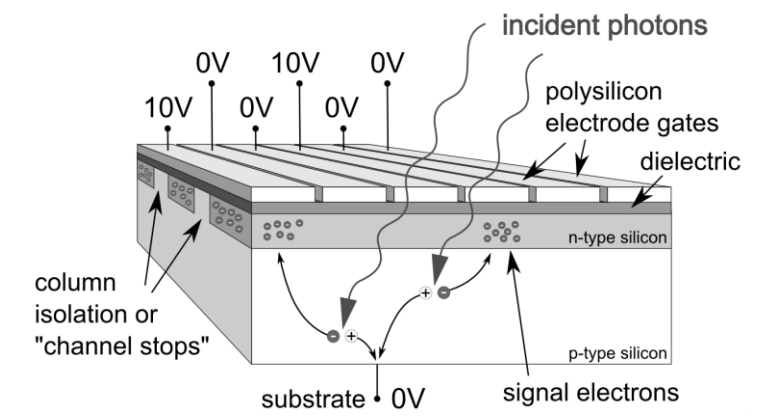
\includegraphics[width=\linewidth,keepaspectratio]{figures/bccd.png}
    \caption{CCD buried channel MOS capacitor\cite{finaltestguideline}}
    \label{fig:mos-cap}
\end{figure}
An imaging sensor is a device that converts an optical image into a digital signal.
%
Charge-coupled devices (CCD) and complementary metal-oxide-semiconductor (CMOS) devices are the most common imaging sensors; CCDs have better performance while CMOS devices are newer and less expensive.

CCDs use densely packed two-dimensional arrays of buried channel\anote{buriedchannel} MOS capacitors (see figure~\ref{fig:mos-cap}) with an individual MOS capacitor being the fundamental photon detecting element.
%
Individual MOS capacitors are biased by a gate voltage such that a signal electron trap (potential well) is produced in the n-type silicon (referred to as the n-channel).
%
When the array is illuminated some of the light is reflected, some is absorbed by the gate, and the rest if transmitted into the silicon.
%
While the absorption coefficients of poly-silicon are fairly high ($4\times 10^4\text{cm}^{-1}$ at 450nm and $1.2\times 10^4\text{cm}^{-1}$ at 550nm) alternative electrode materials exist with better transmission coefficients\cite{Bass:2009:HOT:1594759}.
%
The photons that are transmitted interact with electrons in the valence band of the silicon and excite them into the conduction band, thereby creating electron-hole pairs that either scatter or recombine.
%
For high-quality silicon, the lifetime of such a pair is several milliseconds (before recombination)\cite{scientificccd}.
%
Of those that scatter the electrons move by diffusion into the electron trap while the holes migrate to the substrate (i.e. out of the capacitor).

CCD arrays consist of two sub-arrays: and image section and a readout section.
%
The image section is arranged with every third stripe of electrode tied electrically to form three sets of equipotentials.
\begin{figure}
    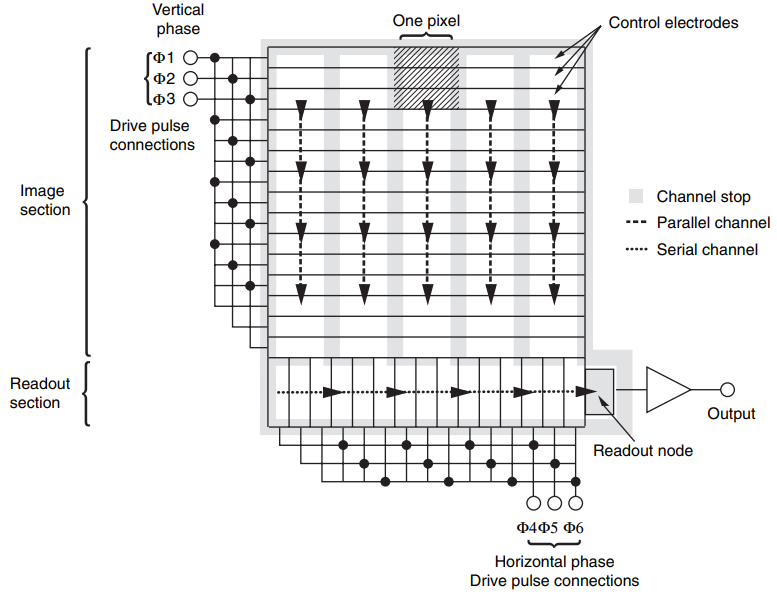
\includegraphics[width=\linewidth,keepaspectratio]{figures/ccd_array.png}
    \caption{CCD array\cite{pawley1995handbook}}
    \label{fig:ccd-array}
\end{figure}
%
In figure ~\ref{fig:ccd-array} these equipotentials are labeled $\Phi1, \Phi2, \Phi3$, and taken together constitute a vertical register (VR).
%
They function to move the collected charge down one line at a time, using charge coupling, while the channel stops function to prevent diffusion of charge across channels.
%
The VR mechanism that moves collected charge functions like this:
\begin{enumerate}
    \item Suppose initially there's a collection of charge on each channel at $\Phi1$ and only $\Phi1$. Note this means $\Phi2$ is at Ov (again just as in figure ~\ref{fig:mos-cap}).
    \item $\Phi2$ is positively biased to 10V. This diffuses the collection of charge under both $\Phi1$ and $\Phi2$.
    \item $\Phi1$ is set to 0v. This concentrates the collection of charge under $\Phi2$.
    \item The same process is repeated with $\Phi2, \Phi3$ and $\Phi3, \Phi1$.
    \item Goto step 1.
\end{enumerate}
At the bottom of the image section $\Phi3$ transfers all signal charges to the horizontal register (HR) which functions much like the VR except much faster: the HR must transfer every line independently of all other lines to the read-out node. For a given image the first pixel read at the read-out node is the bottom-right pixel and the last pixel read is the top-left pixel.

CMOS sensors use
CMOS sensors do not shift charges from row to row; in a CMOS sensor the charge collected in one capacitor is converted to voltage by a circuit integrated into that array element.



%At the beginning of a frame, for each MOS capacitor, a voltage $V_g$ is applied at the gate above the threshold voltage that would ordinarily invert\anote{inversion} the interface between the Si body and the SiO$_2$ (see figure~\ref{fig:inversion}).
%\begin{figure}
%    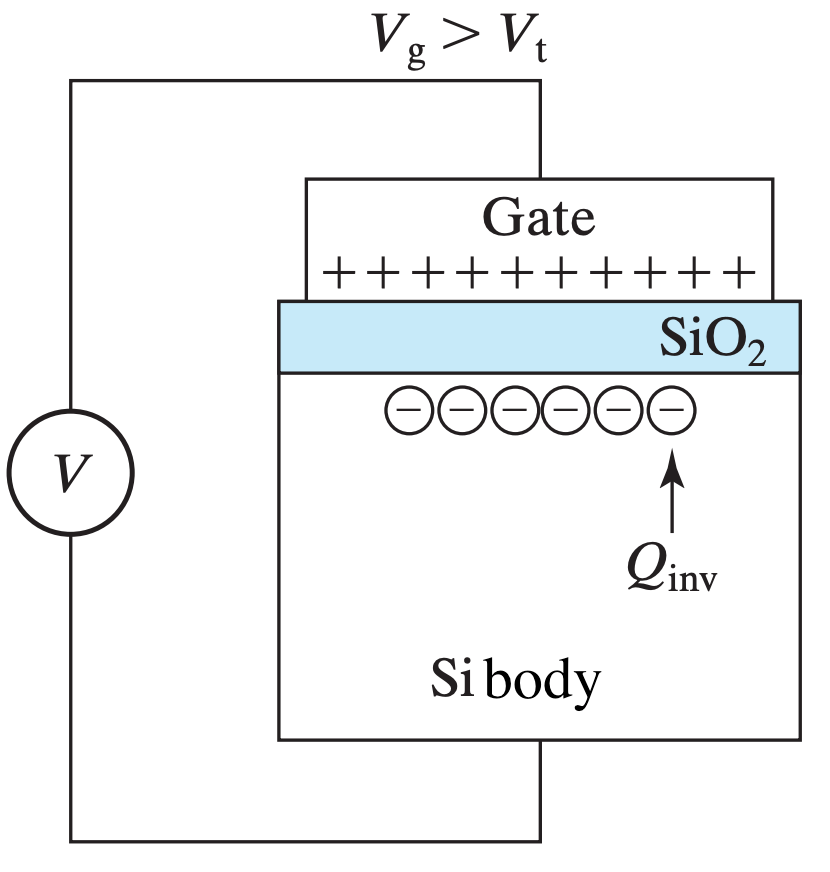
\includegraphics[width=\linewidth,keepaspectratio]{figures/inversion_mos.png}
%    \caption{MOS capacitor biased into deep-depletion\cite{semiconductorbook}}
%    \label{fig:inversion}
%\end{figure}
%As production of inversion electrons is a slow thermal process this leads to \textit{deep-depletion}\anote{deep-depletion} for some fractions of a second.
%%
%If photons are incident on the MOS capacitor during this period photo-generated electron-hole pairs will collect at the interface and the holes will flow through and out of the body.
%%
%The number of such holes is proportional to the number of photons (the intensity of the light).
%
%


\subsection{Mathematical notation}\label{subsec:notation}
Upper case plain latin $X, Y$ denote channel $\times$ row $\times$ column \textit{tensors}\anote{tensor} representing LR and HR images respectively, with $(0,0)$ corresponding to the top left corner of the image.
%
Often for the sake of simplicity we consider greyscale images in which case we omit the channel dimension.
%
Lower case plain latin $x, y$ denote LR and HR \textit{patches}\anote{patch} respectively.
%
$D, H, F, G$ variously refer to functions that operate on images.
%
Bolded latin $\bm{X}, \bm{Y}$ denotes batches.

\subsection{Imaging model}\label{subsec:imaging-model}
Figure~\ref{fig:bertrand} shows a conceptual model of the imaging process as carried out by an imaging system.
%
The input to the system is a natural scene that is in effect sampled by the imaging system.
%
In the idealized case the sampling is done at (or above) the Nyquist rate and no aliasing occurs.
%
In practice there is noise and loss introduced at every step of the process: atmospheric turbulence plays a role at large distances, motion produces multiple views of the same scene but also induces blur, imperfections of the lenses further blur the image, and finally down-sampling by the sensor elements into pixels produces aliasing artifacts\anote{ccd}.
%
The noisy, blurry, down-sampled images are then further degraded by sensor noise.
%
Each such image we call an LR sample.
\begin{figure*}
    \centering
    \begin{adjustbox}{width=\textwidth}
        \begin{tikzpicture}[auto]
            \tikzstyle{terminal} = [rectangle, draw, text width=5em, text centered, minimum height=4em]
            \tikzstyle{block} = [rectangle, draw, fill=gray!20, text width=6em, text centered, rounded corners, minimum height=4em]
            \tikzstyle{line} = [draw, -latex']
            \tikzstyle{sum} = [circle, draw]

            \node[inner sep=0pt] (bertrand) {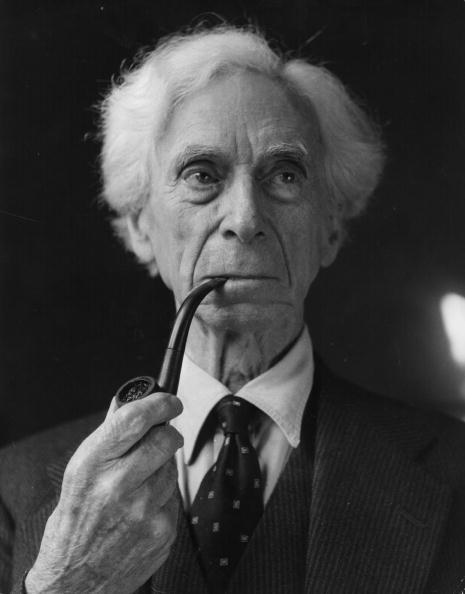
\includegraphics[width=.15\textwidth]{figures/bertrand.png}};
            \node [above = of bertrand] (scene) {Scene};

            \node[sum, right = of bertrand] (sum1) {$+$};
            \node [block, below = of sum1] (atmo-noise) {Atmospheric noise};

            \node [block, right = of sum1] (motion) {Translation, Rotation, Aspect};
            \node [above = of motion] {Motion};

            \node [inner sep=0pt, right = of motion] (motion-output) {};

            \node[inner sep=0pt, below = of motion-output] (bertrand-motion) {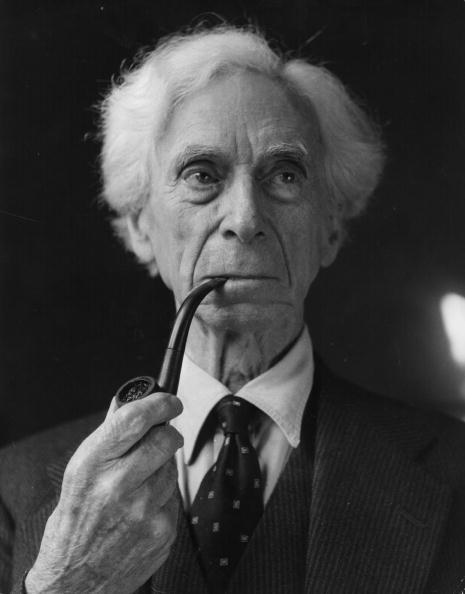
\includegraphics[width=.15\textwidth]{figures/bertrand.png}};
            \node[inner sep=0pt, below = of motion-output, xshift=2mm, yshift=-2mm] {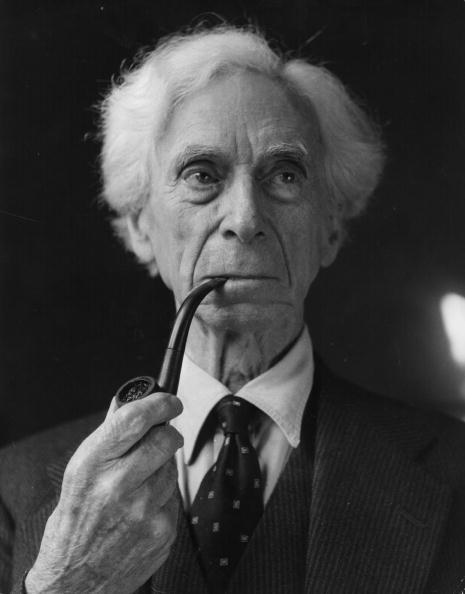
\includegraphics[width=.15\textwidth]{figures/bertrand.png}};
            \node[inner sep=0pt, below = of motion-output, xshift=4mm, yshift=-4mm] {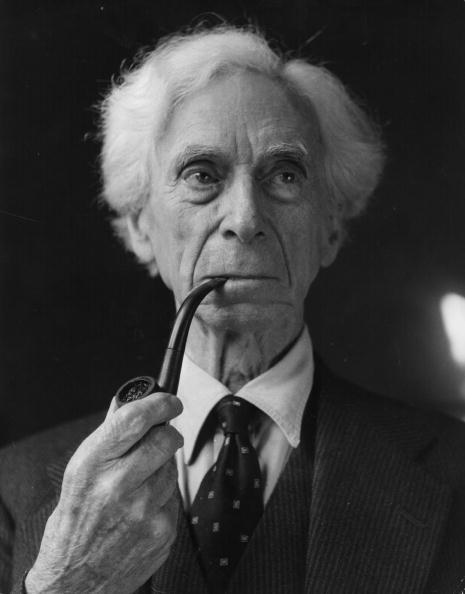
\includegraphics[width=.15\textwidth]{figures/bertrand.png}};
            \node[inner sep=0pt, below = of motion-output, xshift=6mm, yshift=-6mm] {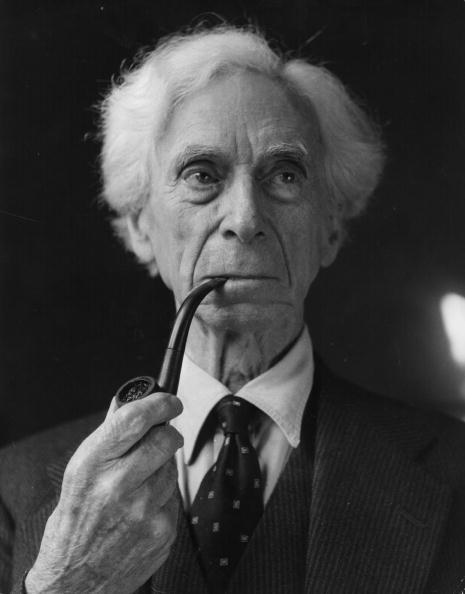
\includegraphics[width=.15\textwidth]{figures/bertrand.png}};

            \node [block, right = of motion-output] (blur) {Optical, Motion};
            \node [above = of blur] {Blur};
            \node [inner sep=0pt, right = of blur] (blur-output) {};

            \node[inner sep=0pt, below = of blur-output] (bertrand-blur) {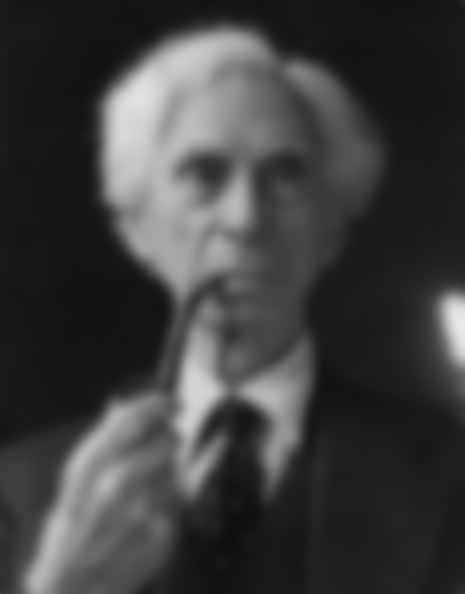
\includegraphics[width=.15\textwidth]{figures/bertrand-blur.png}};
            \node[inner sep=0pt, below = of blur-output, xshift=2mm, yshift=-2mm] {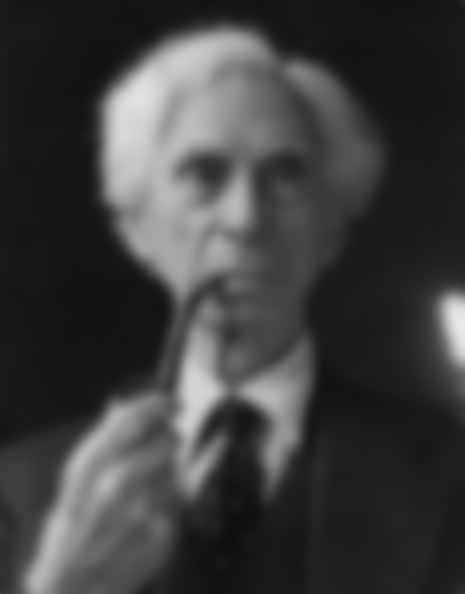
\includegraphics[width=.15\textwidth]{figures/bertrand-blur.png}};
            \node[inner sep=0pt, below = of blur-output, xshift=4mm, yshift=-4mm] {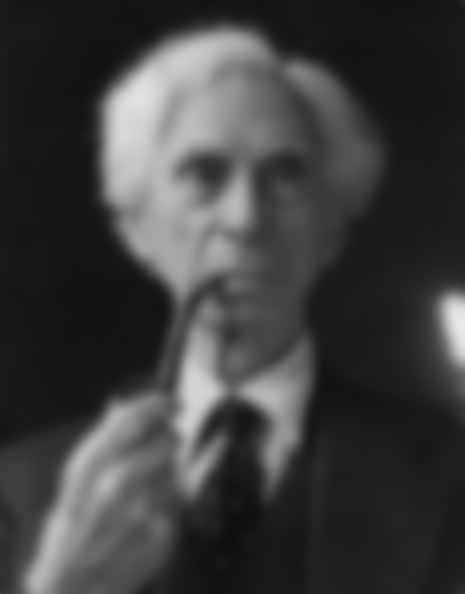
\includegraphics[width=.15\textwidth]{figures/bertrand-blur.png}};
            \node[inner sep=0pt, below = of blur-output, xshift=6mm, yshift=-6mm] {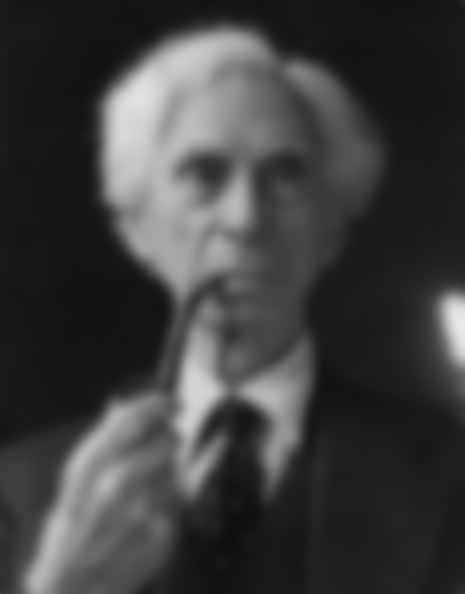
\includegraphics[width=.15\textwidth]{figures/bertrand-blur.png}};

            \node[block, right = of blur-output] (downsample) {Quantization, Pixel-binning};
            \node [above = of downsample] {Down-sampling};

            \node[sum, right = of downsample] (sum2) {$+$};
            \node [block, below = of sum2] (sensor-noise) {Sensor noise};

            \node[inner sep=0pt, right = of sum2] (bertrand-blur-noise) {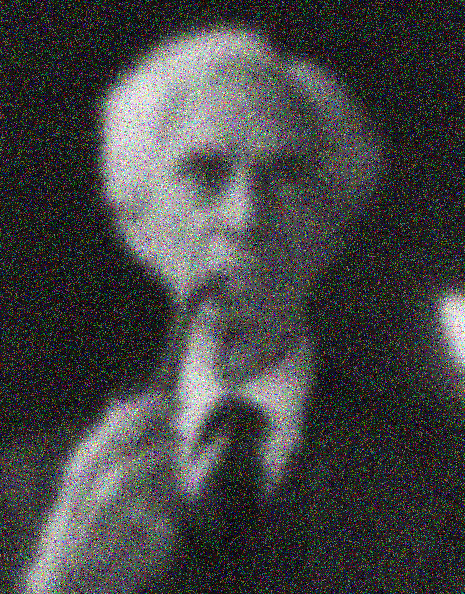
\includegraphics[width=.1\textwidth]{figures/bertrand-blur-noise.png}};
            \node[inner sep=0pt, right = of sum2, xshift=2mm, yshift=-2mm] {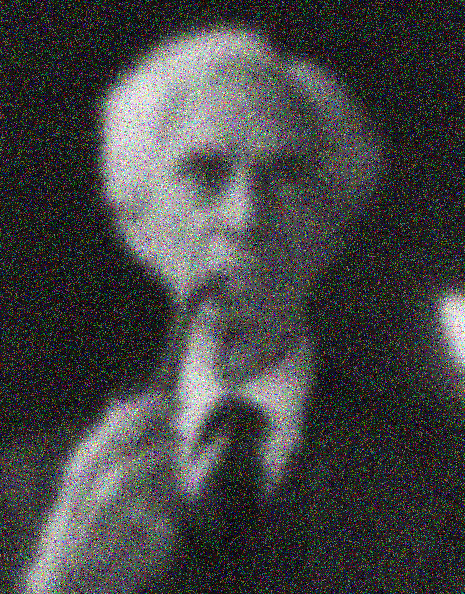
\includegraphics[width=.1\textwidth]{figures/bertrand-blur-noise.png}};
            \node[inner sep=0pt, right = of sum2, xshift=4mm, yshift=-4mm] {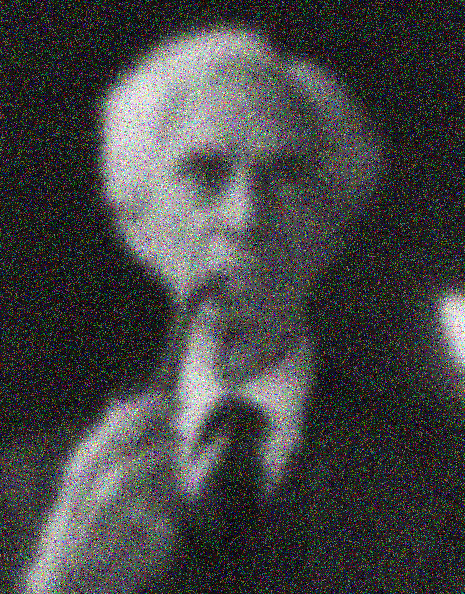
\includegraphics[width=.1\textwidth]{figures/bertrand-blur-noise.png}};
            \node[inner sep=0pt, right = of sum2, xshift=6mm, yshift=-6mm] {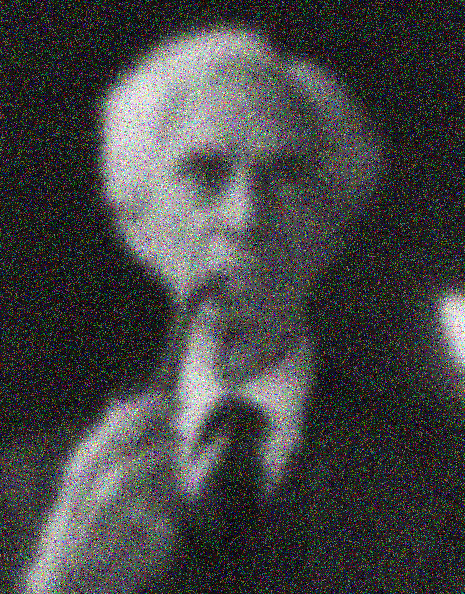
\includegraphics[width=.1\textwidth]{figures/bertrand-blur-noise.png}};
            \node [above = of bertrand-blur-noise, text width=5em] (lr-output) {Low-resolution images};

            \draw[-] (bertrand) edge (sum1);
            \draw[->] (sum1) edge (motion);
            \draw[->] (atmo-noise) edge (sum1);

            \draw[->] (motion) edge (blur);
            \draw[->] (motion-output) edge (bertrand-motion);

            \draw[->] (blur) edge (downsample);
            \draw[->] (blur-output) edge (bertrand-blur);
            \draw[->] (sensor-noise) edge (sum2);
            \draw[-] (downsample) edge (sum2);
            \draw[->] (sum2) edge (bertrand-blur-noise);
        \end{tikzpicture}
    \end{adjustbox}
    \caption{The imaging model illustrating the relationship between a scene and final low-resolution images due to noise, motion, blur, and sampling.}
    \label{fig:bertrand}
\end{figure*}

Let $Y$ denote an idealized HR image of the scene from some fixed vantage point and assume the imaging system collects $K$ LR samples $X_k$ of $Y$.
%
Formally the $X_k$ are related to $Y$ by
\begin{equation}
    X_k = (D_k \circ H_k \circ A_k) (Y) + \epsilon
\end{equation}
where for the $k$th sample $A_k$ is the affine transformation representing motion (rigid and perspective shift), $H_k$ represents the composite blur operator (motion and optics blur), $D_k$ represents the down-sampling operator, and $\epsilon$ represents the composite noise (environment and sensor noise).
%
In general $A_k, H_k, D_k$ are highly degenerate functions for which the corresponding inverse problems are ill-posed without regularization and conditioning.
